
\subsection{Spherical-Earth Reference Solution}
\label{sec:spherical-results}
Starting from the planar solution, we optimize the spherical equations with the same dry mass, propulsion model, touchdown limits, and $15^\circ$ flight-path angle at separation. The best solution we found needs 25.97 t of propellant at separation, 5.77 t of methane and 20.20 t of liquid oxygen, including the 5 t reserve. The booster coasts until 181.3 s, lights its engine at 6.2 km altitude, and touches down at 213.25 s on a ship 284.12 km downrange along the surface.

In the replay at a 0.00125 s step, the booster lands 2.7 mm from the target, moving 0.0028 m/s sideways and 1.507 m/s downward, tilted 0.00034$^\circ$ from vertical and rotating at 0.0129$^\circ$/s. It burns 20.89 t and keeps 5.08 t. Dynamic pressure peaks at 292.9 kPa and specific force at 7.84$\,g_0$.

\paragraph{Speed budget.} In still air, projecting the translational equations along the velocity gives $\dot U=\hat{\mathbf v}\cdot[(\mathbf F_a+\mathbf T)/m-g(h)\hat{\mathbf e}_h]$, where $\hat{\mathbf v}$ is the velocity direction and $\hat{\mathbf e}_h$ is the outward radial direction. The curvature terms cancel in this projection. Integrating these contributions along the replay, aerodynamics removes about 1148 m/s during the coast and gravity adds a net 383 m/s, leaving 901 m/s at ignition. During the burn, aerodynamics removes another 679 m/s and thrust removes 414 m/s, while gravity adds 193 m/s. The remaining speed is about 1.51 m/s. The integral of thrust acceleration magnitude is $\int T/m\,dt=465$ m/s, consistent with Eq.~\eqref{eq:rocket}. Its projection along the velocity accounts for the 414 m/s contribution. Aerodynamic braking therefore supplies most of the speed reduction. The 20.89 t landing burn provides additional braking and brings the booster upright at contact.

Optimization meshes of 0.85, 0.55, and 0.40 s give 26.11, 26.05, 26.04 t, respectively. Three further optimization rounds on the 0.40 s mesh give 26.02, 25.97, 26.01 t; we keep the lowest. Their spread of about 0.05 t shows how precisely the local optimum is resolved. Every reported solution passes the replay at 0.005 and 0.0025 s, and the selected one also at 0.00125 s. The spherical result is 0.26 t lighter than the 26.23 t planar design. Both the trajectory and the controls were reoptimized, so this is the difference between two designs, not a correction applied to one.

Over a 100 s vacuum coast, the integrator conserves specific energy to $7.5\times10^{-9}$ J/kg and angular momentum to a relative error of $6.7\times10^{-16}$. Without torque, the inertial attitude stays constant to $5.9\times10^{-16}$ rad. At 32 sampled states, the derivatives used by the optimizer agree with those of the replay code to within $4.0\times10^{-16}$ after scaling. These tests confirm the signs of the moving-frame terms and the consistency of the two implementations.

\begin{figure}[htbp]\centering
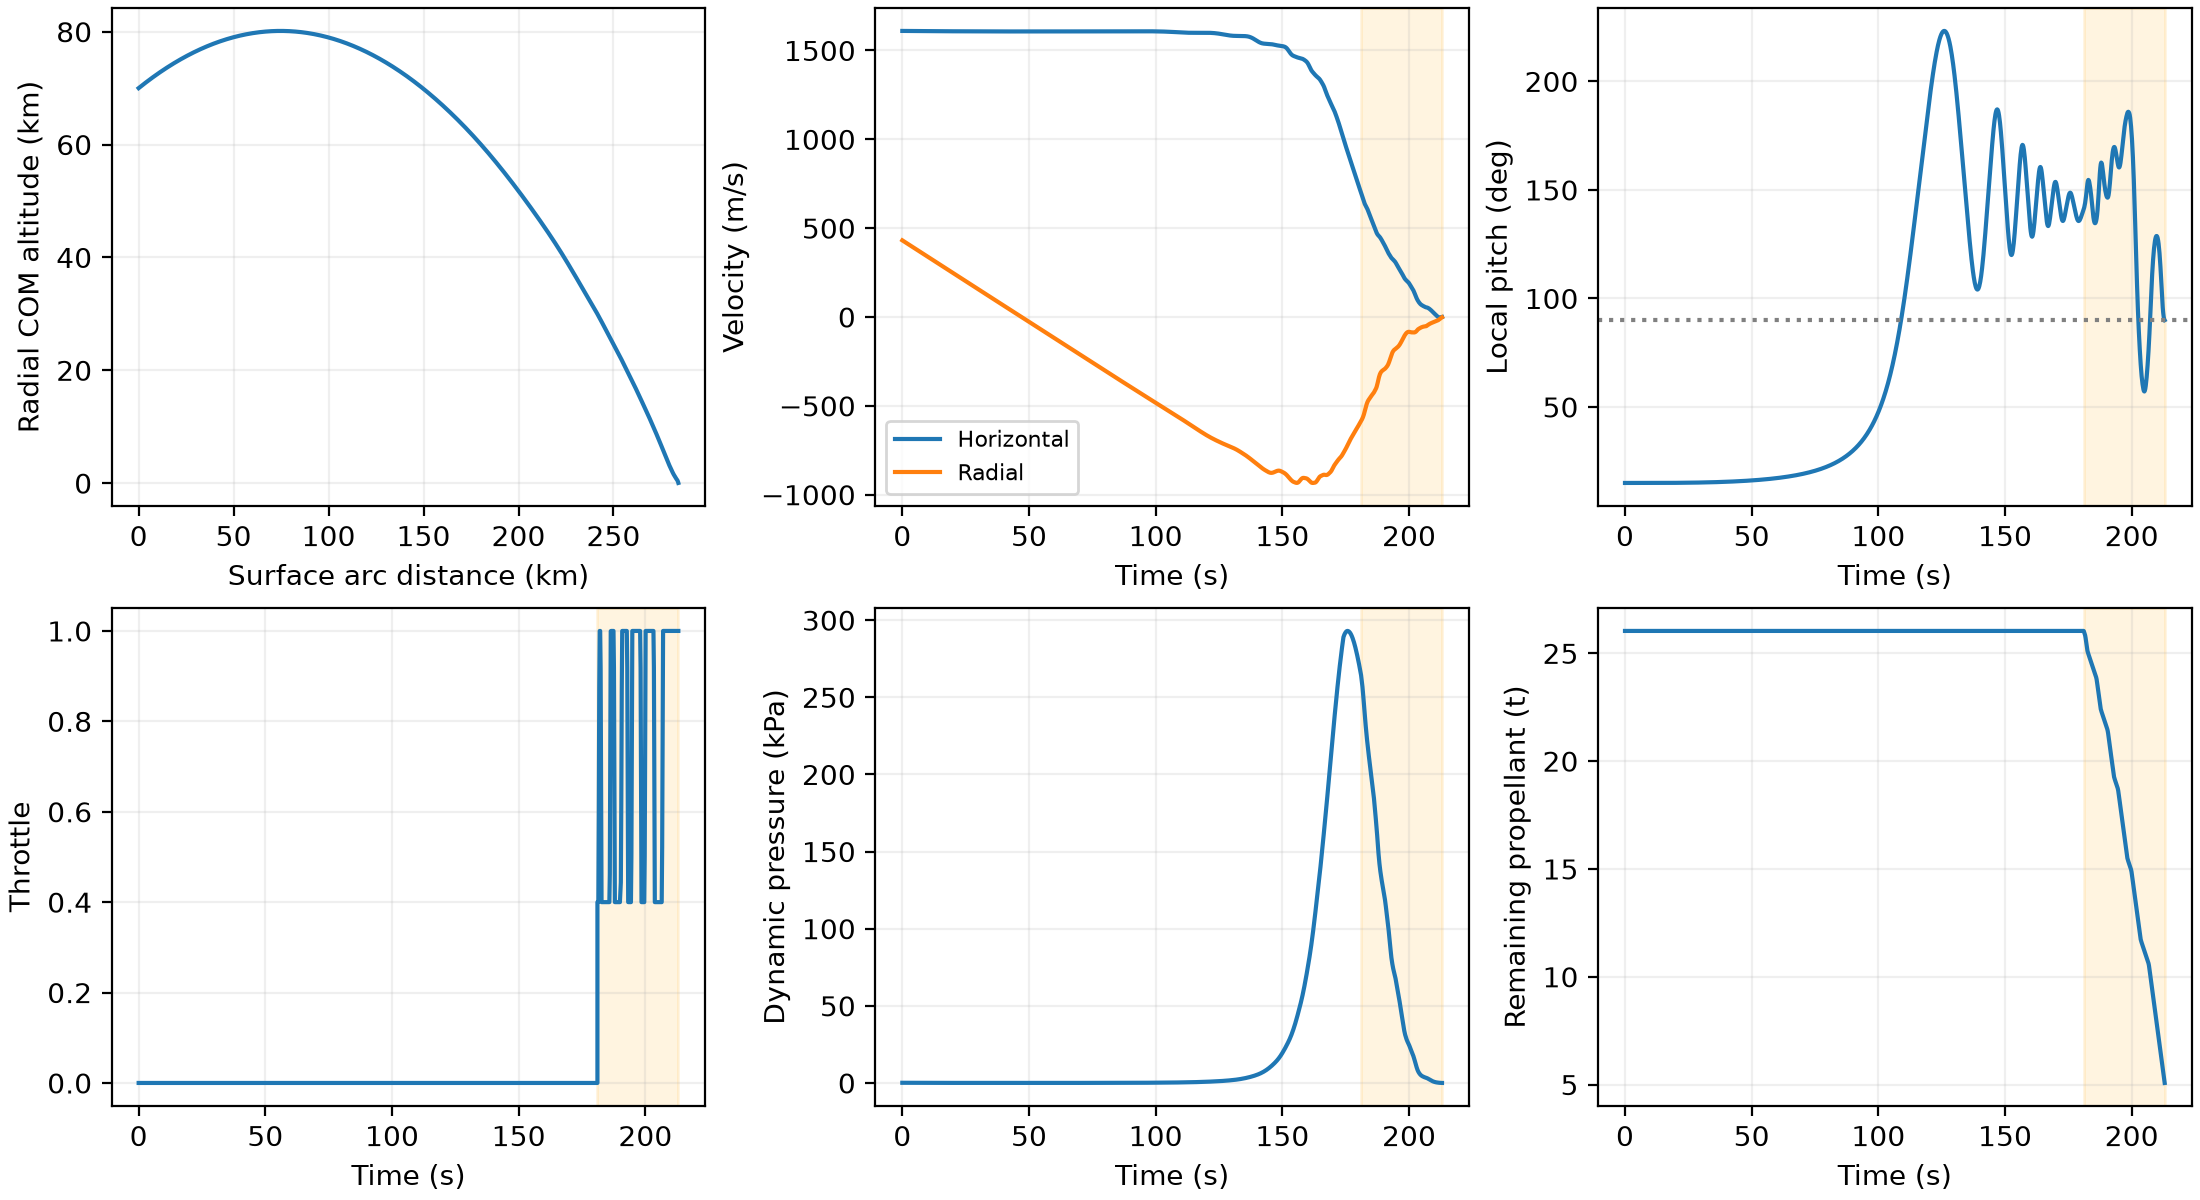
\includegraphics[width=\linewidth]{figure/spherical-reference.png}
\caption{Spherical-Earth reference trajectory. Downrange position is distance along the surface, altitude is radial, and pitch is measured from the local horizontal. Shading marks the landing burn.}
\label{fig:spherical}
\end{figure}
